
\section{Węzły i~sploty}

Wprowadzamy pojęcia węzła i splotu, fundamentalnych obiektów teorii, o której napisana została ta książka.
Oprócz tego podajemy definicję, kiedy dwa węzły lub sploty uznajemy za tożsame oraz uzasadniamy, dlaczego akurat ta definicja jest właściwa.

Istnieją odnogi teorii węzłów, które badają inne, pokrewne obiekty.
Mamy na przykład węzły obramowane:

% DICTIONARY;frame;obramowany;węzeł
% DICTIONARY;framing;obramowanie;-
\begin{definition}[obramowanie]
\index{obramowanie|see {węzeł obramowany}}%
\index{węzeł!obramowany}%
    Każde nieznikające normalne pole wektorowe na splocie nazywamy obramowaniem.
    Jeżeli wszystkie wektory są równoległe do płaszczyzny, na której leży diagram tego splotu, obramowanie nazywamy płaskim\footnote{Po angielsku ,,blackboard framing'', ale nie da się tego sensownie przetłumaczyć...}.
\end{definition}

% Liczba samozaczepienia zorientowanego obramowanego splotu $L$ to indeks zaczepienia tego splotu ze sobą pchniętym w kierunku obramowania, jej wartość to dokładnie spin.

% DICTIONARY;virtual;wirtualny;węzeł
% DICTIONARY;welded;zespawany;węzeł
% DICTIONARY;long;długi;węzeł
Są jeszcze węzły wirtualne, zespawane (iloraz węzłów wirtualnych przez ruch znany jako ,,nadskrzyżowania komutują''), długie (gdzie końce nie są ze sobą zszyte, ale umieszczone tak daleko, że są nieosiągalne) i inne.
\index{węzeł!wirtualny}%
\index{węzeł!zespawany}%
\index{węzeł!długi}%
Ta książka nie zawiera zbyt wiele informacji o wspomnianych bytach.
% TODO wirtualne: 2994594 10.1142/S021821651240007X
% TODO wirtualne: 2191949 https://arxiv.org/pdf/1409.2823.pdf 

\subsection{Węzły}
Matematyczne węzły można traktować jako model elastycznej oraz pozbawionej grubości liny, której luźne końce zostały ze sobą połączone.
Sugeruje to przyjęcie naiwnej definicji:

\begin{definition}[węzeł]
    Ciągłe oraz różnowartościowe odwzorowanie $S^1 \to \R^3$ nazywamy węzłem.
\end{definition}

Takie rozwiązanie nie jest doskonałe, ponieważ oprócz pożądanych (cokolwiek to znaczy) węzłów, obejmuje wiele innych, patologicznych obiektów takich jak ten z~rysunku \ref{fig_wild_knot}.

\begin{figure}[H]
    \centering
\begin{comment}
    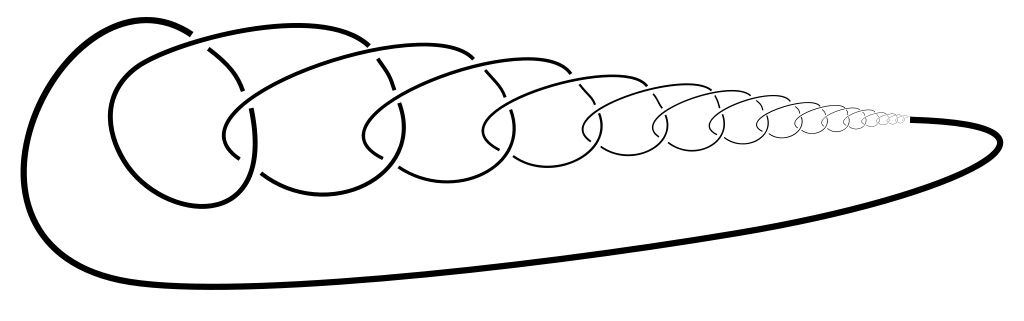
\includegraphics[width=0.44\linewidth]{wild_knot.png}
\end{comment}
    \caption[caption-for-lof-1]{Węzeł dziki, źródło: Wikimedia{\footnotemark}.}
    \label{fig_wild_knot}
\end{figure}
\footnotetext{\url{https://upload.wikimedia.org/wikipedia/commons/2/2f/Wildknot.svg}}

Zamiast wyjaśnić, jakie są jego niepożądane właściwości, podamy od razu dobrą definicję.
Można dodać założenie o tym, że pochodna odwzorowania $S^1 \to \R^3$ nie znika w żadnym punkcie, albo ograniczyć się do łamanych:

\begin{definition}[węzeł]
    Różnowartościowe odwzorowanie $S^1 \to \R^3$, którego pochodna istnieje i nie znika w żadnym punkcie, nazywamy węzłem.
\end{definition}

% DICTIONARY;knot;węzeł;-
% DICTIONARY;tame;poskromiony;węzeł
% DICTIONARY;wild;dziki;węzeł
\begin{definition}[węzeł?]
\index{węzeł}%
\label{def:knot}%
    Gładkie włożenie $S^1 \to \R^3$ otaczająco izotopijne z~zamkniętą łamaną bez samoprzecięć nazywamy węzłem poskromionym.
    Dwa węzły są równoważne, jeśli istnieje pomiędzy nimi izotopia otaczająca.
\end{definition}
% TODO: potrzeba jednocześnie gładkości i łamanych?

Czasami wygodniej jest rozpatrywać węzeł jako włożenie $S^1 \to S^3$ albo dopuścić do myśli węzły nieposkromione.
Ale jeśli nie zaznaczono inaczej, nie robimy tego: pisząc węzeł mamy na myśli poskromione włożenie w przestrzeń $\R^3$, nie $S^3$.

Potrzeba jeszcze matematycznego opisu manipulacji, jakim możemy poddawać sznur trzymany w ręce.
Izotopia jest niewłaściwym narzędziem do tego celu: powiedzielibyśmy, że dwa węzły $K_1, K_2$ sa izotopijne, jeśli istnieje ciągła funkcja $F \colon S^1 \times [0, 1] \to \R^3$ taka, że $K_1 = F(-, 0)$ jest pierwszym, zaś $K_2 = F(-,1)$ drugim węzłem (funkcję $F$ nazywa się izotopia).
Tym razem źródło problemów można wskazać jawnie.
Sztuczka Alexandera pozwala usunąć dowolny zaplątany fragment z węzła:

% https://i.stack.imgur.com/QlTxR.png
\begin{figure}[H]
    \centering
\begin{comment}
    
\includegraphics[width=0.44\linewidth]{../data/missing.jpg}
\end{comment}
    \caption[caption-for-lof-2]{Sztuczka? Alexandera??}
\end{figure}

W podobny sposób moglibyśmy przekształcić dowolny węzeł w~niewęzeł.
Teoria, w~której wszystkie obiekty są takie same, nie jest zbyt ciekawa.
Od izotopii należy wymagać gładkości albo lokalnej płaskości,
% https://math.stackexchange.com/questions/1311865/equivalence-of-knots-ambient-isotopy-vs-homeomorphism
co zdaje się prowadzić do pojęcia izotopii otaczającej, która uwzględnia nie tylko sam węzły, ale też to, jak leżą w otaczającej je przestrzeni.

% DICTIONARY;isotopy;izotopia;-
% DICTIONARY;ambient;otaczająca;izotopia
\begin{definition}[izotopia otaczająca]
\index{izotopia otaczająca}%
    Niech $N, M$ będą rozmaitościami, zaś $K_1, K_2 \colon N \to M$ włożeniami.
    Ciągłe odwzorowanie $F \colon M \times [0,1] \to M$ spełniające następujące warunki:
    \begin{enumerate}
        \item funkcja $F(-, 0)$ jest odwzorowaniem tożsamościowym,
        \item każda z funkcji $F(-, t)$ jest homeomorfizmem,
        \item złożenie $F(-, 1)$ z pierwszym włożeniem $K_1$ daje drugie włożenie $K_2$
    \end{enumerate}
    nazywamy izotopią otaczającą przenoszącą $K_1$ na $K_2$.
\end{definition}

W topologii rozważa się włożenia dowolnych rozmaitości, nam wystarczy jeden szczególny przypadek $N = S^1$ oraz $M = \R^3$.
Intuicyjnie, funkcja $F$ zniekształca przestrzeń $\R^3$ tak, że w~chwili początkowej $t = 0$ widzimy pierwszy, zaś w~chwili końcowej $t = 1$ drugi węzeł.
Izotopia otaczająca nie pozwala na ściąganie zaplątanych fragmentów do punktu.

Formalnie węzły to pewne odwzorowania, więc prawidłowym sposobem na zapisanie, że są izotopijne (czyli dla nas: równe), jest $K_1 \cong K_2$.
Ponieważ nie prowadzi to do problemów, będziemy jednak stosować zapis $K_1 = K_2$.
Jednocześnie często węzeł jako odwzorowanie nie będzie odróżniany od obrazu tego odwzorowania.

Istnieje jeszcze jedna, konkurencyjna definicja węzłów równoważnych:

\begin{proposition}
\label{def:equivalent_knots_2}%
    Dwa węzły są równoważne wtedy i tylko wtedy, gdy jeden z~nich jest obrazem drugiego przez zachowujący orientację homeomorfizm $\R^3 \to \R^3$.
\end{proposition}

\begin{proof}
\index[persons]{Milnor, John}%
    Podany niżej dowód pochodzi z~książki ,,Topology from the differentiable viewpoint'' Johna Milnora\footnote{John Willard Milnor zajmuje się głównie topologią różniczkową oraz algebraiczną K-teorią; jego główne dokonania w świecie węzłów to wprowadzenie niezmienników Milnora, które uogólniają grupę podstawową dopełnienia oraz pewne wyniki dotyczące hipotezy plastrowo-taśmowej.}.
\index[persons]{Milnor, John}%
    Musimy pokazać, że dyfeomorfizm $f \colon \R^m \to \R^m$ jest gładko izotopijny z~identycznością.
    Translacje są izotopiami, więc bez straty ogólności zakładamy, że $f(0) = 0$.
    Pochodna $f$ w~zerze jest dana wzorem $\mathrm{d}f_0(x) = \lim_{t \to 0} f(tx) /t$,
    naturalną definicję izotopii $F \colon \R^m \times [0, 1] \to \R^m$ stanowi więc
    \begin{equation}
        F(x, t) = \begin{cases}
            \mathrm{d}f_0(x) & t = 0 \\
            f(tx) / t & 0 < t \le 1
        \end{cases} .
    \end{equation}

    Na mocy lematu Hadamarda funkcja $f$ zapisuje się jako suma $x_1 g_1(x) + \ldots + x_mg_m(x)$, gdzie funkcje $g_i$ są gładkie, więc funkcja $F$ też jest gładka, co jakoś kończy dowód.
\end{proof}

Milnor zauważa, że istnieje dyfeomorfizm $S^6 \to S^6$ stopnia $+1$, który nie jest gładko izotopijny z~identycznością!

\subsection{Sploty}
% DICTIONARY;link;splot;-
% DICTIONARY;component;ogniwo splotu;-
\begin{definition}[splot, ogniwo]
\index{splot}%
    Sumę parami rozłącznych węzłów
    \begin{equation}
        L = K_1 \sqcup K_2 \sqcup \ldots K_n
    \end{equation}
    nazywamy splotem, a~składniki sumy -- ogniwami.
\end{definition}

Przez analogię do węzłów mówimy, że dwa sploty są takie same, jeśli jeden jest obrazem drugiego przez zachowujący orientację homeomorfizm $\R^3 \to \R^3$.
W~takiej sytuacji obydwa sploty mają tyle samo ogniw.

\begin{example}
\index{splot!Hopfa}%
\index[persons]{Hopf, Heinz}%
    Splot Hopfa\footnote{Heinz Hopf był niemiecko-szwajcarskim pionierem topologii algebraicznej. W~1931 roku zajmował się splotem Hopfa w ramach badań nad tzw. rozwłóknieniem \emph{(Hopf fibration)}.} to najprostszy splot nietrywialny.
\end{example}

\begin{example}
\index{splot!Whiteheada}%
\index[persons]{Whitehead, John}%
    Splot Whiteheada\footnote{John Henry Constantine Whitehead był jednym z założycieli teorii homotopii. Oprócz wspomnianego tu splotu Whiteheada zobaczymy jego nazwisko jeszcze raz, przy dublu Whiteheada.} ma dwa ogniwa i w~1934 służył Whiteheadowi za kontrprzykład do nieudanego dowodu (także Whiteheada!) hipotezy Poincarego.
\end{example}

\begin{comment}
    \begin{figure}[H]
        \begin{minipage}[b]{.48\linewidth}
            \centering
            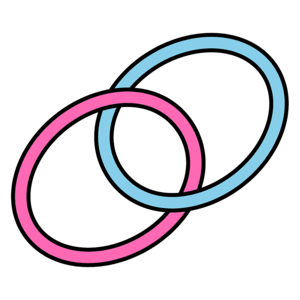
\includegraphics[width=0.5\linewidth]{../data/links/2_2_1.png}
            \subcaption{splot Hopfa}
        \end{minipage}
        \begin{minipage}[b]{.48\linewidth}
            \centering
            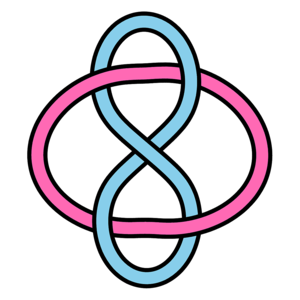
\includegraphics[width=0.5\linewidth]{../data/links/5_2_1.png}
            \subcaption{splot Whiteheada}
        \end{minipage}
    \end{figure}
\end{comment}

% TODO: przesunąć to gdzieś dalej, za definicję skrzyżowania
Poniższa definicja nie jest nam jeszcze potrzebna, ale wygodnie przytoczyć ją już teraz.

% DICTIONARY;splittable;rozszczepialny;splot
\begin{definition}[rozszczepialność]
\index{splot!rozszczepialny}%
    Jeżeli splot $L$ można zanurzyć w przestrzeni $\R^3$ tak, że niektóre jego ogniwa będą leżeć nad pewną rozłączną ze splotem płaszczyzną, zaś pozostałe pod nią, to powiemy, że splot $L$ jest rozszczepialny.
\end{definition}

Liczbę nierozszczepialnych splotów pierwszych zebrano w~tabeli:

\renewcommand*{\arraystretch}{1.4}
\footnotesize
\begin{longtable}{lcccccccccccc}
    \hline
    \textbf{skrzyżowania} & 0 & 1 & 2 & 3 & 4 & 5 &  6 &  7 &  8 & 9 & 10 & 11 \\ \hline \endhead
    sploty pierwsze, nierozszczepialne & 0 & 0 & 1 & 0 & 1 & 1 & 6 & 9 & 29 & 83 & 287 & 1007 \\
    (w tym) alternujące & 0 & 0 & 1 & 0 & 1 & 1 & 5 & 7 & 21 & 55 & 174 & 548 \\
    (w tym) niealternujące & 0 & 0 & 0 & 0 & 0 & 0 & 1 & 2 & 8 & 28 & 113 & 459 \\
    \hline
\end{longtable}
\normalsize

W bazie danych OEIS można trafić na ciąg \href{https://oeis.org/A086826}{A086826} opisujący liczbę nierozszczepialnych pierwszych i złożonych węzłów i splotów.
Powyższa tabela zawiera liczby na podstawie portalu LinkInfo \cite{linkinfo24}.
Odpowiedź na pytanie ,,czym są skrzyżowania?'' przynosi definicja \ref{def:crossing}.

Pewne kryteria rozszczepialności konkretnych splotów znaleźć można u Kawauchiego \cite[s. 36-38]{kawauchi96}.

\subsection{Dopełnienia węzłów i splotów}

Jeśli dwa węzły są równoważne, to ich dopełnienia są oczywiście homeomorficzne.
Pytanie o~prawdziwość implikacji odwrotnej jako pierwszy zadał najprawdopodobniej Tietze \cite{tietze08} w~1908 roku.
\index[persons]{Tietze, Heinrich}%
W roku 1987 pokazano, że istnieją co najwyżej dwa węzły o~zadanym dopełnieniu (Culler, Gordon, Luecke, Shalen \cite{culler87}).
\index[persons]{Culler, Marc}%
\index[persons]{Shalen, Peter}%
\index[persons]{Gordon, Cameron}%
\index[persons]{Luecke, John}%
Dwa lata później poznaliśmy pozytywną odpowiedź na pytanie Tietzego: każdy węzeł jest wyznaczony jednoznacznie przez swoje dopełnienie.

\begin{theorem}[Gordon, Luecke, 1989]
\index[persons]{Gordon, Cameron}%
\index[persons]{Luecke, John}%
\index{twierdzenie!Gordona-Lueckego}%
    Poskromione węzły o~homeomorficznych (z zachowaniem orientacji) dopełnieniach są wzajemnie izotopijne.
\end{theorem}

\begin{proof}[Niedowód]
    Wynika to z teorii Cerfa, kombinatorycznych technik w stylu Litherlanda, cienkich pozycji, cykli Scharlemanna i~ogólniejszego stwierdzenia: nietrywialna chirurgia Dehna na węźle w~3-sferze nigdy nie daje 3-sfery.
% https://en.wikipedia.org/wiki/Gordon–Luecke_theorem: Essential ingredients of the proof are their joint work with Marc Culler and Peter Shalen on the cyclic surgery theorem, combinatorial techniques in the style of Litherland, thin position, and Scharlemann cycles.
\index{chirurgia Dehna}%
\index{teoria Cerfa}%
\index{cykle Scharlemanna}%
    Pełny dowód zawiera praca \cite{gordon89}.
\end{proof}

Twierdzenie to zamienia problem lokalny (czy dwa węzły w kuli $S^3$ są równoważne?) na problem globalny (czy dwie przestrzenie topologiczne są homeomorficzne?).
Jego odpowiednik dla splotów jest fałszywy i wiedziano o tym od bardzo dawna: w~1937 roku Whitehead \cite{whitehead37} podał nieskończenie wiele splotów, których dopełnienia wyglądają jak dopełnienia splotu Whiteheada.
\index[persons]{Whitehead, John}%

% koniec sekcji Węzły i sploty

